\hypertarget{temperature__sensor___terciopelo_8pde}{
\section{/Users/nikki/nublabs/nub.datalogger/hardware/temperature\_\-sensor\_\-Terciopelo/temperature\_\-sensor\_\-Terciopelo.pde File Reference}
\label{temperature__sensor___terciopelo_8pde}\index{/Users/nikki/nublabs/nub.datalogger/hardware/temperature\_\-sensor\_\-Terciopelo/temperature\_\-sensor\_\-Terciopelo.pde@{/Users/nikki/nublabs/nub.datalogger/hardware/temperature\_\-sensor\_\-Terciopelo/temperature\_\-sensor\_\-Terciopelo.pde}}
}
{\tt \#include \char`\"{}name.h\char`\"{}}\par
{\tt \#include \char`\"{}globals.h\char`\"{}}\par
{\tt \#include \char`\"{}communications\_\-definitions.h\char`\"{}}\par
{\tt \#include $<$stdio.h$>$}\par


Include dependency graph for temperature\_\-sensor\_\-Terciopelo.pde:\nopagebreak
\begin{figure}[H]
\begin{center}
\leavevmode
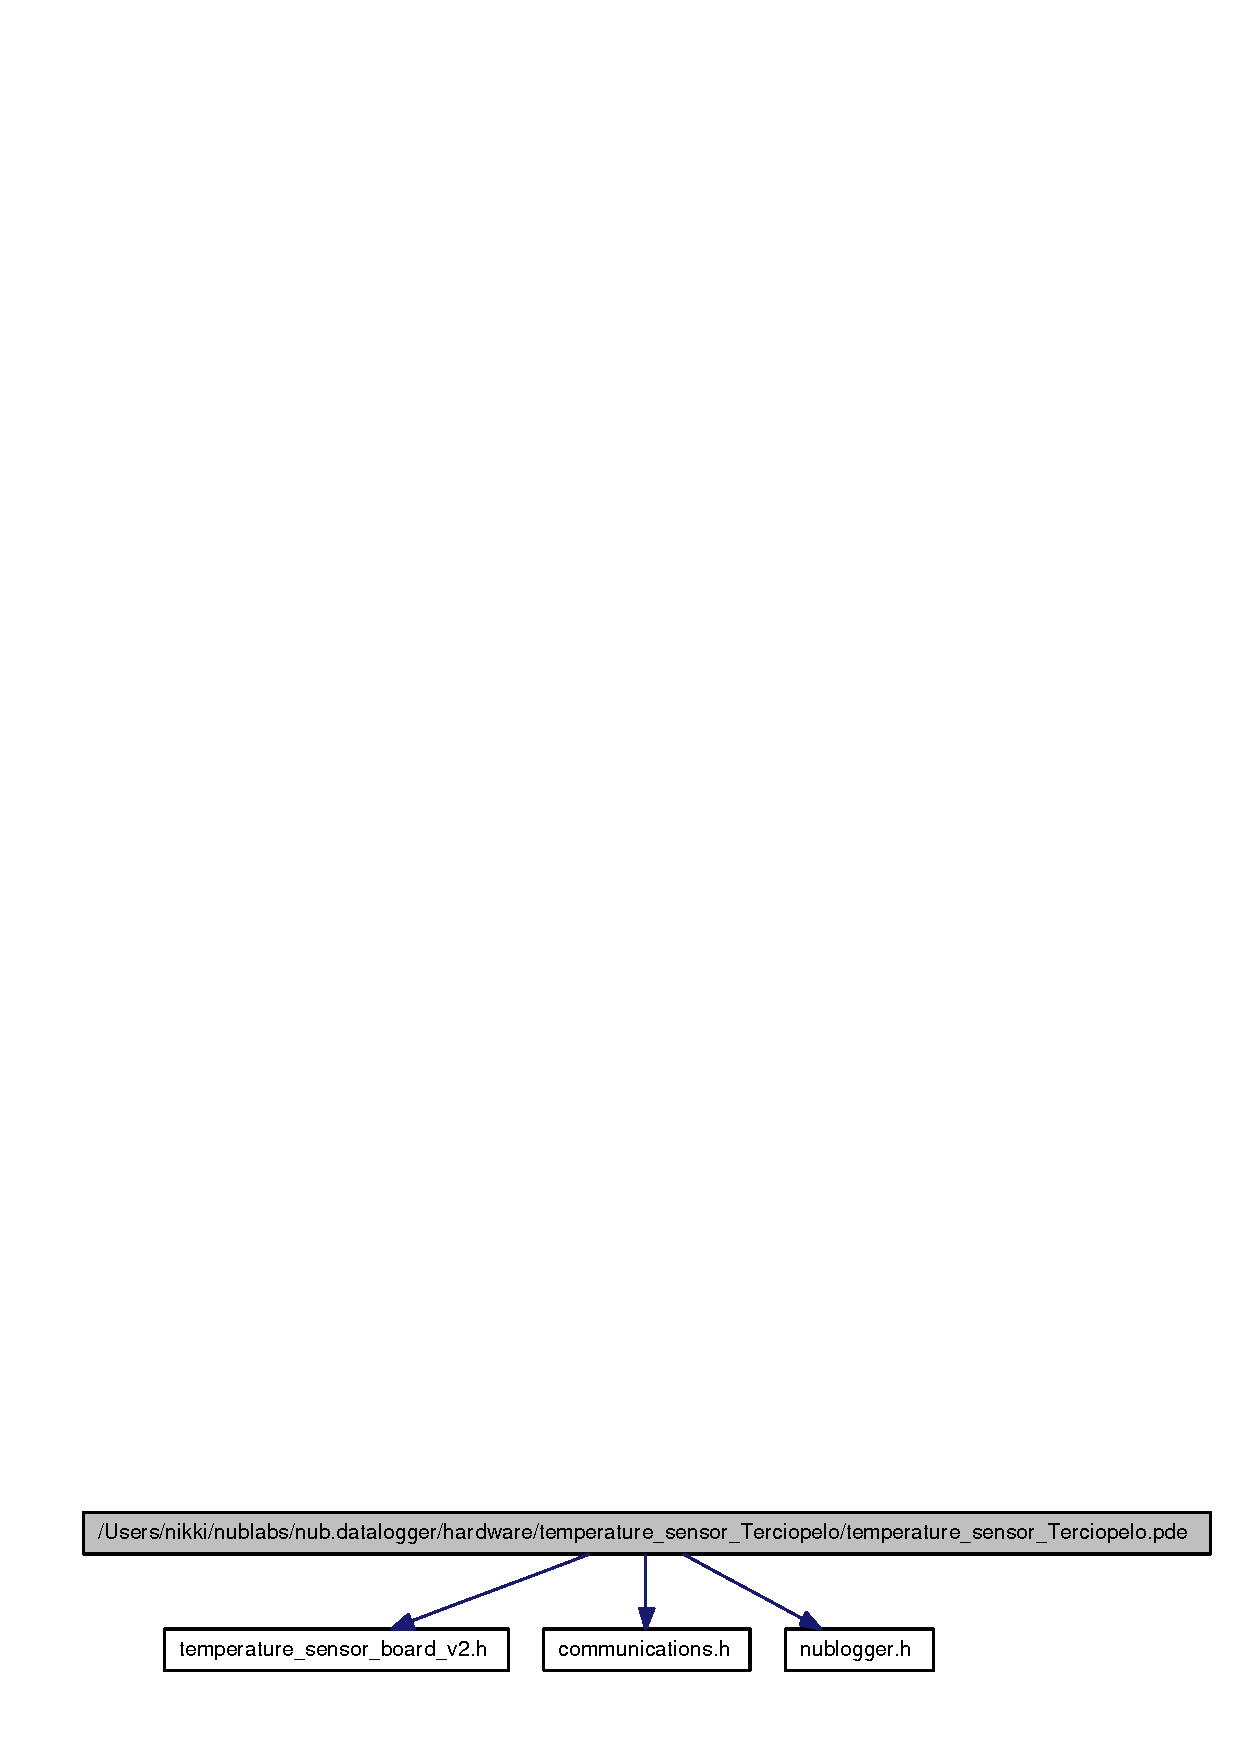
\includegraphics[width=292pt]{temperature__sensor___terciopelo_8pde__incl}
\end{center}
\end{figure}
\subsection*{Defines}
\begin{CompactItemize}
\item 
\#define \hyperlink{temperature__sensor___terciopelo_8pde_658c2878485cfe5cc625d283a6d34bc1}{XBEE\_\-SLEEP}~2
\item 
\#define \hyperlink{temperature__sensor___terciopelo_8pde_b2de299215608c2a35f0feb86adc2f6f}{SAMPLE\_\-BUTTON}~3
\item 
\#define \hyperlink{temperature__sensor___terciopelo_8pde_eb7a7ba1ab7e0406f1b5ab36d579f585}{LED}~4
\item 
\#define \hyperlink{temperature__sensor___terciopelo_8pde_2a2946288d28852ba343b09fd4f17d7a}{SENSOR1\_\-TOP}~0
\item 
\#define \hyperlink{temperature__sensor___terciopelo_8pde_0da2a51dcb3e00b10aedd07d75f22382}{SENSOR1\_\-BOTTOM}~1
\item 
\#define \hyperlink{temperature__sensor___terciopelo_8pde_645141ae2ab7fa7ac3f690c4959b6baf}{SENSOR2\_\-TOP}~2
\item 
\#define \hyperlink{temperature__sensor___terciopelo_8pde_df66e6da6cf8c78004dc0a75fd14d3b1}{SENSOR2\_\-BOTTOM}~3
\end{CompactItemize}
\subsection*{Functions}
\begin{CompactItemize}
\item 
void \hyperlink{temperature__sensor___terciopelo_8pde_4fc01d736fe50cf5b977f755b675f11d}{setup} ()
\item 
void \hyperlink{temperature__sensor___terciopelo_8pde_fe461d27b9c48d5921c00d521181f12f}{loop} ()
\item 
void \hyperlink{temperature__sensor___terciopelo_8pde_50a2ce599e896bfb535e70a42003ed23}{sample} ()
\item 
int \hyperlink{temperature__sensor___terciopelo_8pde_f8c68e93feeba5b9244094043672bac0}{getByte} (int timeout)
\item 
int \hyperlink{temperature__sensor___terciopelo_8pde_8f2521044963073c55b3c290fffd79e3}{getMessage} (int timeout)
\item 
void \hyperlink{temperature__sensor___terciopelo_8pde_95b1b253ee46df6a93285803cf1f3370}{sendData} ()
\begin{CompactList}\small\item\em this function takes care of putting together a message string, calculating a checksum, sending it out to the computer and making sure the computer got it ok \item\end{CompactList}\item 
unsigned char \hyperlink{temperature__sensor___terciopelo_8pde_465a79dc430d1e52a5b540920da744ca}{getChecksum} ()
\begin{CompactList}\small\item\em this computes a checksum of the global string 'message' \item\end{CompactList}\item 
void \hyperlink{temperature__sensor___terciopelo_8pde_e369b3765489ee8bd0ea791c1843630f}{configure} ()
\begin{CompactList}\small\item\em \hyperlink{nublogger_8h_e369b3765489ee8bd0ea791c1843630f}{configure()} runs if the computer is trying to change the sensor's sample rate \item\end{CompactList}\item 
void \hyperlink{temperature__sensor___terciopelo_8pde_3fdb2350c3f98c0de0f0ae3c831a8b14}{discover} ()
\begin{CompactList}\small\item\em This function tells the computer of the datalogger's existence. \item\end{CompactList}\item 
void \hyperlink{temperature__sensor___terciopelo_8pde_b4dbd8380e5d93ead613cf38e6083b7f}{waitForSampleInterval} ()
\begin{CompactList}\small\item\em this function waits for the time specified by the global variables 'hours,' 'minutes,' and 'seconds' It should ideally put the arduino in a power saving mode \item\end{CompactList}\item 
void \hyperlink{temperature__sensor___terciopelo_8pde_f6c9587ccbcf223f8c79f508c2fef366}{initializeSensor} ()
\begin{CompactList}\small\item\em this function configures all the digital communication pins as input or output pins \item\end{CompactList}\item 
void \hyperlink{temperature__sensor___terciopelo_8pde_a06edc5122b70b3231ff87d8234fe759}{xbeeSleep} ()
\item 
void \hyperlink{temperature__sensor___terciopelo_8pde_884c5dd8e3bb500063c819db197db666}{xbeeWake} ()
\item 
void \hyperlink{temperature__sensor___terciopelo_8pde_ea28af0c7128421a38589128bb39ef1c}{getTemperatures} ()
\item 
void \hyperlink{temperature__sensor___terciopelo_8pde_cfc975251dbc3a8c9a9b11f8df62cc41}{getRawData} ()
\begin{CompactList}\small\item\em this just grabs the raw values off the analog to digital converter \item\end{CompactList}\item 
void \hyperlink{temperature__sensor___terciopelo_8pde_8e666a34a083b1806167ca991be0c436}{convertToResistance} ()
\begin{CompactList}\small\item\em this function converts the raw ADC values from the thermistor into resistances of the thermistor \item\end{CompactList}\item 
void \hyperlink{temperature__sensor___terciopelo_8pde_3aa4f99331713009a70ee34eba83754b}{convertToTemperature} ()
\end{CompactItemize}
\subsection*{Variables}
\begin{CompactItemize}
\item 
float \hyperlink{temperature__sensor___terciopelo_8pde_735577560ca40e5b6008a98829068904}{R0} = 10000.0
\item 
float \hyperlink{temperature__sensor___terciopelo_8pde_8188fea1f6709096fe21a3ee084d00d0}{B} = 3950.0
\item 
float \hyperlink{temperature__sensor___terciopelo_8pde_4211ba1269f650e21964d32238a460b2}{T0} = 298
\item 
float \hyperlink{temperature__sensor___terciopelo_8pde_d17df5990b551ac9e97a3d60f65833ff}{RBOTTOM} = 1000.0
\end{CompactItemize}


\subsection{Define Documentation}
\hypertarget{temperature__sensor___terciopelo_8pde_eb7a7ba1ab7e0406f1b5ab36d579f585}{
\index{temperature\_\-sensor\_\-Terciopelo.pde@{temperature\_\-sensor\_\-Terciopelo.pde}!LED@{LED}}
\index{LED@{LED}!temperature_sensor_Terciopelo.pde@{temperature\_\-sensor\_\-Terciopelo.pde}}
\subsubsection[{LED}]{\setlength{\rightskip}{0pt plus 5cm}\#define LED~4}}
\label{temperature__sensor___terciopelo_8pde_eb7a7ba1ab7e0406f1b5ab36d579f585}




Definition at line 323 of file temperature\_\-sensor\_\-Terciopelo.pde.\hypertarget{temperature__sensor___terciopelo_8pde_b2de299215608c2a35f0feb86adc2f6f}{
\index{temperature\_\-sensor\_\-Terciopelo.pde@{temperature\_\-sensor\_\-Terciopelo.pde}!SAMPLE\_\-BUTTON@{SAMPLE\_\-BUTTON}}
\index{SAMPLE\_\-BUTTON@{SAMPLE\_\-BUTTON}!temperature_sensor_Terciopelo.pde@{temperature\_\-sensor\_\-Terciopelo.pde}}
\subsubsection[{SAMPLE\_\-BUTTON}]{\setlength{\rightskip}{0pt plus 5cm}\#define SAMPLE\_\-BUTTON~3}}
\label{temperature__sensor___terciopelo_8pde_b2de299215608c2a35f0feb86adc2f6f}




Definition at line 322 of file temperature\_\-sensor\_\-Terciopelo.pde.\hypertarget{temperature__sensor___terciopelo_8pde_0da2a51dcb3e00b10aedd07d75f22382}{
\index{temperature\_\-sensor\_\-Terciopelo.pde@{temperature\_\-sensor\_\-Terciopelo.pde}!SENSOR1\_\-BOTTOM@{SENSOR1\_\-BOTTOM}}
\index{SENSOR1\_\-BOTTOM@{SENSOR1\_\-BOTTOM}!temperature_sensor_Terciopelo.pde@{temperature\_\-sensor\_\-Terciopelo.pde}}
\subsubsection[{SENSOR1\_\-BOTTOM}]{\setlength{\rightskip}{0pt plus 5cm}\#define SENSOR1\_\-BOTTOM~1}}
\label{temperature__sensor___terciopelo_8pde_0da2a51dcb3e00b10aedd07d75f22382}




Definition at line 326 of file temperature\_\-sensor\_\-Terciopelo.pde.\hypertarget{temperature__sensor___terciopelo_8pde_2a2946288d28852ba343b09fd4f17d7a}{
\index{temperature\_\-sensor\_\-Terciopelo.pde@{temperature\_\-sensor\_\-Terciopelo.pde}!SENSOR1\_\-TOP@{SENSOR1\_\-TOP}}
\index{SENSOR1\_\-TOP@{SENSOR1\_\-TOP}!temperature_sensor_Terciopelo.pde@{temperature\_\-sensor\_\-Terciopelo.pde}}
\subsubsection[{SENSOR1\_\-TOP}]{\setlength{\rightskip}{0pt plus 5cm}\#define SENSOR1\_\-TOP~0}}
\label{temperature__sensor___terciopelo_8pde_2a2946288d28852ba343b09fd4f17d7a}




Definition at line 325 of file temperature\_\-sensor\_\-Terciopelo.pde.\hypertarget{temperature__sensor___terciopelo_8pde_df66e6da6cf8c78004dc0a75fd14d3b1}{
\index{temperature\_\-sensor\_\-Terciopelo.pde@{temperature\_\-sensor\_\-Terciopelo.pde}!SENSOR2\_\-BOTTOM@{SENSOR2\_\-BOTTOM}}
\index{SENSOR2\_\-BOTTOM@{SENSOR2\_\-BOTTOM}!temperature_sensor_Terciopelo.pde@{temperature\_\-sensor\_\-Terciopelo.pde}}
\subsubsection[{SENSOR2\_\-BOTTOM}]{\setlength{\rightskip}{0pt plus 5cm}\#define SENSOR2\_\-BOTTOM~3}}
\label{temperature__sensor___terciopelo_8pde_df66e6da6cf8c78004dc0a75fd14d3b1}




Definition at line 328 of file temperature\_\-sensor\_\-Terciopelo.pde.\hypertarget{temperature__sensor___terciopelo_8pde_645141ae2ab7fa7ac3f690c4959b6baf}{
\index{temperature\_\-sensor\_\-Terciopelo.pde@{temperature\_\-sensor\_\-Terciopelo.pde}!SENSOR2\_\-TOP@{SENSOR2\_\-TOP}}
\index{SENSOR2\_\-TOP@{SENSOR2\_\-TOP}!temperature_sensor_Terciopelo.pde@{temperature\_\-sensor\_\-Terciopelo.pde}}
\subsubsection[{SENSOR2\_\-TOP}]{\setlength{\rightskip}{0pt plus 5cm}\#define SENSOR2\_\-TOP~2}}
\label{temperature__sensor___terciopelo_8pde_645141ae2ab7fa7ac3f690c4959b6baf}




Definition at line 327 of file temperature\_\-sensor\_\-Terciopelo.pde.\hypertarget{temperature__sensor___terciopelo_8pde_658c2878485cfe5cc625d283a6d34bc1}{
\index{temperature\_\-sensor\_\-Terciopelo.pde@{temperature\_\-sensor\_\-Terciopelo.pde}!XBEE\_\-SLEEP@{XBEE\_\-SLEEP}}
\index{XBEE\_\-SLEEP@{XBEE\_\-SLEEP}!temperature_sensor_Terciopelo.pde@{temperature\_\-sensor\_\-Terciopelo.pde}}
\subsubsection[{XBEE\_\-SLEEP}]{\setlength{\rightskip}{0pt plus 5cm}\#define XBEE\_\-SLEEP~2}}
\label{temperature__sensor___terciopelo_8pde_658c2878485cfe5cc625d283a6d34bc1}


these are the pin definitions for the v2 board

function atmega pin arduino pin

Serial RX PD0 0 //serial lines that go out to the xbee module Serial TX PD1 1 Xbee\_\-sleep PD2 2 //a pin that, when asserted, puts the xbee radio into a low power sleep mode Sample\_\-button PD3 3 //an optional button that forces the sensor to take and send out a measurement LED PD4 4 //an LED on board that you can use for all kinds of stuff

sensor1\_\-top PC0 (analog) 0 sensor1\_\-bottom PC1 (analog) 1 sensor2\_\-top PC2 (analog) 2 sensor2\_\-bottom PC3 (analog) 3 

Definition at line 321 of file temperature\_\-sensor\_\-Terciopelo.pde.

\subsection{Function Documentation}
\hypertarget{temperature__sensor___terciopelo_8pde_e369b3765489ee8bd0ea791c1843630f}{
\index{temperature\_\-sensor\_\-Terciopelo.pde@{temperature\_\-sensor\_\-Terciopelo.pde}!configure@{configure}}
\index{configure@{configure}!temperature_sensor_Terciopelo.pde@{temperature\_\-sensor\_\-Terciopelo.pde}}
\subsubsection[{configure}]{\setlength{\rightskip}{0pt plus 5cm}void configure ()}}
\label{temperature__sensor___terciopelo_8pde_e369b3765489ee8bd0ea791c1843630f}


\hyperlink{nublogger_8h_e369b3765489ee8bd0ea791c1843630f}{configure()} runs if the computer is trying to change the sensor's sample rate 

In \hyperlink{nublogger_8h_e369b3765489ee8bd0ea791c1843630f}{configure()}, the datalogger sends a LISTENING message to the computer, indicating that it's ready to receive data. The computer sends three ints: the hours, minutes and seconds of the sample interval, followed by a checksum byte that's the sum of the ints modulo 256. The sensor computes a checksum on the received data. If its checksum matches, it sends an ACKNOWLEDGE message back to the computer and updates its sample interval information. If the checksum does not match, it sends a CHECKSUM\_\-ERROR\_\-PLEASE\_\-RESEND message, asking the computer to send the three ints again, followed by a checksum. If the sensor can't get a valid message (with a matching checksum) after three tries, it gives up, sends a CHECKSUM\_\-ERROR\_\-GIVING\_\-UP message to the computer and keeps its original sample interval information 

Definition at line 183 of file temperature\_\-sensor\_\-Terciopelo.pde.

References buffer, CHECKSUM, CHECKSUM\_\-ERROR\_\-GIVING\_\-UP, CHECKSUM\_\-ERROR\_\-PLEASE\_\-RESEND, CONFIGURATION\_\-MESSAGE\_\-LENGTH, configured, getMessage(), HOUR\_\-HIGH, HOUR\_\-LOW, hours, index, LISTENING, MALFORMED\_\-MESSAGE\_\-ERROR\_\-GIVING\_\-UP, MALFORMED\_\-MESSAGE\_\-ERROR\_\-PLEASE\_\-RESEND, MESSAGE\_\-START, MINUTE\_\-HIGH, MINUTE\_\-LOW, minutes, NUM\_\-TRIES, SECOND\_\-HIGH, SECOND\_\-LOW, seconds, start, and TIMEOUT\_\-ERROR.

\begin{Code}\begin{verbatim}184 { 
185   char i=0;
186   char tries=0;
187   char success=0;
188   unsigned char checksum=0;
189   int error;
190   
191   while((tries<NUM_TRIES)&&(success==0))     //we'll try
192   {
193   checksum=0;
194   Serial.print(LISTENING,BYTE);
195   error=getMessage(100);
196   if(error==-1)
197     Serial.print(TIMEOUT_ERROR,BYTE);
198   else
199   {
200     if(buffer[start]==MESSAGE_START)
201     {
202       if((index-start)==CONFIGURATION_MESSAGE_LENGTH)    //check to make sure the message is the size we expect
203       {
204         for(i=1;i<CHECKSUM;i++)
205           checksum+=buffer[start+i];
206         if(checksum==buffer[start+CHECKSUM])    //check to see if the calculated checksum is the same as the received checksum
207         {
208           //if it is, then we can load all the sample interval info
209           hours=(int)buffer[start+HOUR_HIGH]*256+(int)buffer[start+HOUR_LOW];
210           minutes=(int)buffer[start+MINUTE_HIGH]*256+(int)buffer[start+MINUTE_LOW];
211           seconds=(int)buffer[start+SECOND_HIGH]*256+(int)buffer[start+SECOND_LOW];
212           success=1;         //we can stop looping
213           configured=1;      //the sensor is configured!
214         }
215         else
216         {
217           if(tries<NUM_TRIES)
218           {
219             Serial.print(CHECKSUM_ERROR_PLEASE_RESEND);
220             tries++;
221           }
222           else
223             Serial.print(CHECKSUM_ERROR_GIVING_UP);
224         }
225       }
226       else      //the message is the wrong size
227         {
228           if(tries<NUM_TRIES)
229           {
230             Serial.print(MALFORMED_MESSAGE_ERROR_PLEASE_RESEND);
231             tries++;
232           }
233           else
234             Serial.print(MALFORMED_MESSAGE_ERROR_GIVING_UP);
235         }
236     }
237     else
238         {
239           if(tries<NUM_TRIES)
240           {
241             Serial.print(MALFORMED_MESSAGE_ERROR_PLEASE_RESEND);
242             tries++;
243           }
244           else
245             Serial.print(MALFORMED_MESSAGE_ERROR_GIVING_UP);
246         }
247   }
248   }
249 }
\end{verbatim}
\end{Code}


\hypertarget{temperature__sensor___terciopelo_8pde_8e666a34a083b1806167ca991be0c436}{
\index{temperature\_\-sensor\_\-Terciopelo.pde@{temperature\_\-sensor\_\-Terciopelo.pde}!convertToResistance@{convertToResistance}}
\index{convertToResistance@{convertToResistance}!temperature_sensor_Terciopelo.pde@{temperature\_\-sensor\_\-Terciopelo.pde}}
\subsubsection[{convertToResistance}]{\setlength{\rightskip}{0pt plus 5cm}void convertToResistance ()}}
\label{temperature__sensor___terciopelo_8pde_8e666a34a083b1806167ca991be0c436}


this function converts the raw ADC values from the thermistor into resistances of the thermistor 



Definition at line 383 of file temperature\_\-sensor\_\-Terciopelo.pde.

References RBOTTOM, sensor1\_\-bottom, sensor1\_\-resistance, and sensor1\_\-top.

Referenced by getTemperatures().

\begin{Code}\begin{verbatim}384 {
385     sensor1_resistance = ((float)sensor1_top/(float)sensor1_bottom - 1)*RBOTTOM; // Voltages converted to resistances
386     /* uncomment if I enable two sensing elements
387     sensor2_resistance = ((float)sensor2_top/(float)sensor2_bottom - 1)*RBOTTOM; // Voltages converted to resistances*/
388  
389 }
\end{verbatim}
\end{Code}


\hypertarget{temperature__sensor___terciopelo_8pde_3aa4f99331713009a70ee34eba83754b}{
\index{temperature\_\-sensor\_\-Terciopelo.pde@{temperature\_\-sensor\_\-Terciopelo.pde}!convertToTemperature@{convertToTemperature}}
\index{convertToTemperature@{convertToTemperature}!temperature_sensor_Terciopelo.pde@{temperature\_\-sensor\_\-Terciopelo.pde}}
\subsubsection[{convertToTemperature}]{\setlength{\rightskip}{0pt plus 5cm}void convertToTemperature ()}}
\label{temperature__sensor___terciopelo_8pde_3aa4f99331713009a70ee34eba83754b}




Definition at line 392 of file temperature\_\-sensor\_\-Terciopelo.pde.

References B, R0, sensor1\_\-resistance, sensor1\_\-temperature, and T0.

Referenced by getTemperatures(), and sample().

\begin{Code}\begin{verbatim}393 {
394    sensor1_temperature = float(B/log(sensor1_resistance/(R0*exp(-1.0*B/T0))) - 273.0); // Temperature in degrees Celsius
395    /* uncomment if I enable two sensing elements
396    sensor2_temperature = float(B/log(sensor2_resistance/(R0*exp(-1.0*B/T0))) - 273.0); // Temperature in degrees Celsius   */
397 }
\end{verbatim}
\end{Code}


\hypertarget{temperature__sensor___terciopelo_8pde_3fdb2350c3f98c0de0f0ae3c831a8b14}{
\index{temperature\_\-sensor\_\-Terciopelo.pde@{temperature\_\-sensor\_\-Terciopelo.pde}!discover@{discover}}
\index{discover@{discover}!temperature_sensor_Terciopelo.pde@{temperature\_\-sensor\_\-Terciopelo.pde}}
\subsubsection[{discover}]{\setlength{\rightskip}{0pt plus 5cm}void discover ()}}
\label{temperature__sensor___terciopelo_8pde_3fdb2350c3f98c0de0f0ae3c831a8b14}


This function tells the computer of the datalogger's existence. 

When the sensor turns on, it runs \hyperlink{nublogger_8h_3fdb2350c3f98c0de0f0ae3c831a8b14}{discover()}. It sends a MESSAGE\_\-START message, a DISCOVER\_\-ME message, and its name out to the computer and waits for acknowledgement. The computer can send back a plain \char`\"{}ACKNOWLEDGE\char`\"{} message, which means that the sensor should run using its default configuration values. The computer can also send back an \char`\"{}ACKNOWLEDGE\_\-AND\_\-CONFIGURE\char`\"{} message, which means that it has configuration data for the sensor. If the sensor gets this message, it'll run \hyperlink{nublogger_8h_e369b3765489ee8bd0ea791c1843630f}{configure()} to receive the data from the computer. 

Definition at line 260 of file temperature\_\-sensor\_\-Terciopelo.pde.

References ACKNOWLEDGE, ACKNOWLEDGE\_\-AND\_\-CONFIGURE, configure(), DISCOVER\_\-ME, discovered, getByte(), MESSAGE\_\-END, MESSAGE\_\-START, name, TIMEOUT\_\-ERROR, and TRUE.

\begin{Code}\begin{verbatim}261 { 
262   unsigned char checksum=0;
263   int i=0;
264   Serial.print(MESSAGE_START, BYTE);
265   Serial.print(DISCOVER_ME,BYTE);
266   Serial.print(name);
267   while(name[i]!=0)
268   {
269     checksum+=name[i];
270     i++;
271   }
272   checksum+=DISCOVER_ME;
273   Serial.print(checksum,BYTE);
274   Serial.print(MESSAGE_END,BYTE);
275 
276   int receivedByte=getByte(100);     //looks for a byte on the serial port with a 100ms timeout
277   if(receivedByte==ACKNOWLEDGE)
278     discovered=TRUE;
279   if(receivedByte==ACKNOWLEDGE_AND_CONFIGURE)
280     {
281       discovered=TRUE;
282       configure();
283     }
284   if(receivedByte==-1)
285   {
286     Serial.print(TIMEOUT_ERROR,BYTE);  //getByte didn't get a byte before the timeout
287   }  
288 }
\end{verbatim}
\end{Code}


\hypertarget{temperature__sensor___terciopelo_8pde_f8c68e93feeba5b9244094043672bac0}{
\index{temperature\_\-sensor\_\-Terciopelo.pde@{temperature\_\-sensor\_\-Terciopelo.pde}!getByte@{getByte}}
\index{getByte@{getByte}!temperature_sensor_Terciopelo.pde@{temperature\_\-sensor\_\-Terciopelo.pde}}
\subsubsection[{getByte}]{\setlength{\rightskip}{0pt plus 5cm}int getByte (int {\em timeout})}}
\label{temperature__sensor___terciopelo_8pde_f8c68e93feeba5b9244094043672bac0}




Definition at line 94 of file temperature\_\-sensor\_\-Terciopelo.pde.

\begin{Code}\begin{verbatim}95 {
96   int currentTime=millis();
97   int maxTime=currentTime+timeout;
98   while((Serial.available()==0)&&(millis()<(maxTime)))
99     {}
100   if(Serial.available()>0)        //did any data come in on the serial port?
101     return Serial.read();
102   else                             //we didn't get any data before the timeout
103     return -1;
104 }
\end{verbatim}
\end{Code}


\hypertarget{temperature__sensor___terciopelo_8pde_465a79dc430d1e52a5b540920da744ca}{
\index{temperature\_\-sensor\_\-Terciopelo.pde@{temperature\_\-sensor\_\-Terciopelo.pde}!getChecksum@{getChecksum}}
\index{getChecksum@{getChecksum}!temperature_sensor_Terciopelo.pde@{temperature\_\-sensor\_\-Terciopelo.pde}}
\subsubsection[{getChecksum}]{\setlength{\rightskip}{0pt plus 5cm}unsigned char getChecksum ()}}
\label{temperature__sensor___terciopelo_8pde_465a79dc430d1e52a5b540920da744ca}


this computes a checksum of the global string 'message' 



Definition at line 159 of file temperature\_\-sensor\_\-Terciopelo.pde.

References message.

Referenced by sendData().

\begin{Code}\begin{verbatim}160 {
161   char i=0;
162   unsigned char checksum=0;
163   while(message[i]!=0)
164   {
165     checksum+=message[i];
166     i++;
167   }
168   return checksum;
169 }
\end{verbatim}
\end{Code}


\hypertarget{temperature__sensor___terciopelo_8pde_8f2521044963073c55b3c290fffd79e3}{
\index{temperature\_\-sensor\_\-Terciopelo.pde@{temperature\_\-sensor\_\-Terciopelo.pde}!getMessage@{getMessage}}
\index{getMessage@{getMessage}!temperature_sensor_Terciopelo.pde@{temperature\_\-sensor\_\-Terciopelo.pde}}
\subsubsection[{getMessage}]{\setlength{\rightskip}{0pt plus 5cm}int getMessage (int {\em timeout})}}
\label{temperature__sensor___terciopelo_8pde_8f2521044963073c55b3c290fffd79e3}




Definition at line 106 of file temperature\_\-sensor\_\-Terciopelo.pde.

References buffer, index, MESSAGE\_\-END, and start.

Referenced by configure().

\begin{Code}\begin{verbatim}107 {
108   int completeMessage=-1;   //a flag that lets us know if we got a full message
109   start=index;              //drop whatever other data is in our buffer--it'll probably just confuse the functions if we don't
110   int currentTime=millis();
111   int maxTime=currentTime+timeout;  
112   while((millis()<(maxTime))&&(buffer[index]!=MESSAGE_END))
113     {
114       if(Serial.available()>0)
115         {
116           buffer[index]=Serial.read();
117           if(buffer[index]==MESSAGE_END)   //we got a complete message
118             completeMessage=1;
119           index++;
120         }
121     }
122   if(completeMessage==-1)    //we never got a complete message
123     start=index;    //skip past whatever we got from the buffer
124   
125   return completeMessage;
126 }
\end{verbatim}
\end{Code}


\hypertarget{temperature__sensor___terciopelo_8pde_cfc975251dbc3a8c9a9b11f8df62cc41}{
\index{temperature\_\-sensor\_\-Terciopelo.pde@{temperature\_\-sensor\_\-Terciopelo.pde}!getRawData@{getRawData}}
\index{getRawData@{getRawData}!temperature_sensor_Terciopelo.pde@{temperature\_\-sensor\_\-Terciopelo.pde}}
\subsubsection[{getRawData}]{\setlength{\rightskip}{0pt plus 5cm}void getRawData ()}}
\label{temperature__sensor___terciopelo_8pde_cfc975251dbc3a8c9a9b11f8df62cc41}


this just grabs the raw values off the analog to digital converter 



Definition at line 372 of file temperature\_\-sensor\_\-Terciopelo.pde.

References sensor1\_\-bottom, and sensor1\_\-top.

Referenced by getTemperatures(), and sample().

\begin{Code}\begin{verbatim}373 {
374   sensor1_top=analogRead(0);
375   sensor1_bottom=analogRead(1);
376   
377 /*  uncomment if I enable 2-sensing elements per sensor
378   sensor2_top=analogRead(2);
379   sensor2_bottom=analogRead(3);*/
380 }
\end{verbatim}
\end{Code}


\hypertarget{temperature__sensor___terciopelo_8pde_ea28af0c7128421a38589128bb39ef1c}{
\index{temperature\_\-sensor\_\-Terciopelo.pde@{temperature\_\-sensor\_\-Terciopelo.pde}!getTemperatures@{getTemperatures}}
\index{getTemperatures@{getTemperatures}!temperature_sensor_Terciopelo.pde@{temperature\_\-sensor\_\-Terciopelo.pde}}
\subsubsection[{getTemperatures}]{\setlength{\rightskip}{0pt plus 5cm}void getTemperatures ()}}
\label{temperature__sensor___terciopelo_8pde_ea28af0c7128421a38589128bb39ef1c}




Definition at line 364 of file temperature\_\-sensor\_\-Terciopelo.pde.

References convertToResistance(), convertToTemperature(), and getRawData().

\begin{Code}\begin{verbatim}365 {
366   getRawData();
367   convertToResistance();
368   convertToTemperature();
369 }
\end{verbatim}
\end{Code}


\hypertarget{temperature__sensor___terciopelo_8pde_f6c9587ccbcf223f8c79f508c2fef366}{
\index{temperature\_\-sensor\_\-Terciopelo.pde@{temperature\_\-sensor\_\-Terciopelo.pde}!initializeSensor@{initializeSensor}}
\index{initializeSensor@{initializeSensor}!temperature_sensor_Terciopelo.pde@{temperature\_\-sensor\_\-Terciopelo.pde}}
\subsubsection[{initializeSensor}]{\setlength{\rightskip}{0pt plus 5cm}void initializeSensor ()}}
\label{temperature__sensor___terciopelo_8pde_f6c9587ccbcf223f8c79f508c2fef366}


this function configures all the digital communication pins as input or output pins 

If you adapt this code to work with another sensor or board, you should replace the code in \hyperlink{temperature__sensor__board__v2_8h_f6c9587ccbcf223f8c79f508c2fef366}{initializeSensor()} to initialize all your relevant pins 

Definition at line 343 of file temperature\_\-sensor\_\-Terciopelo.pde.

References LED, SAMPLE\_\-BUTTON, XBEE\_\-SLEEP, and xbeeWake().

\begin{Code}\begin{verbatim}344  {
345    pinMode(XBEE_SLEEP,OUTPUT);
346    pinMode(SAMPLE_BUTTON,INPUT);
347    pinMode(LED,OUTPUT);
348    xbeeWake();
349  }  
\end{verbatim}
\end{Code}


\hypertarget{temperature__sensor___terciopelo_8pde_fe461d27b9c48d5921c00d521181f12f}{
\index{temperature\_\-sensor\_\-Terciopelo.pde@{temperature\_\-sensor\_\-Terciopelo.pde}!loop@{loop}}
\index{loop@{loop}!temperature_sensor_Terciopelo.pde@{temperature\_\-sensor\_\-Terciopelo.pde}}
\subsubsection[{loop}]{\setlength{\rightskip}{0pt plus 5cm}void loop ()}}
\label{temperature__sensor___terciopelo_8pde_fe461d27b9c48d5921c00d521181f12f}




Definition at line 79 of file temperature\_\-sensor\_\-Terciopelo.pde.

References sample(), and waitForSampleInterval().

\begin{Code}\begin{verbatim}80 {
81   waitForSampleInterval();
82   sample();
83 }
\end{verbatim}
\end{Code}


\hypertarget{temperature__sensor___terciopelo_8pde_50a2ce599e896bfb535e70a42003ed23}{
\index{temperature\_\-sensor\_\-Terciopelo.pde@{temperature\_\-sensor\_\-Terciopelo.pde}!sample@{sample}}
\index{sample@{sample}!temperature_sensor_Terciopelo.pde@{temperature\_\-sensor\_\-Terciopelo.pde}}
\subsubsection[{sample}]{\setlength{\rightskip}{0pt plus 5cm}void sample ()}}
\label{temperature__sensor___terciopelo_8pde_50a2ce599e896bfb535e70a42003ed23}




Definition at line 85 of file temperature\_\-sensor\_\-Terciopelo.pde.

References convertToTemperature(), getRawData(), and sendData().

Referenced by loop().

\begin{Code}\begin{verbatim}86 {
87   getRawData();
88   convertToTemperature();
89   sendData();
90 }
\end{verbatim}
\end{Code}


\hypertarget{temperature__sensor___terciopelo_8pde_95b1b253ee46df6a93285803cf1f3370}{
\index{temperature\_\-sensor\_\-Terciopelo.pde@{temperature\_\-sensor\_\-Terciopelo.pde}!sendData@{sendData}}
\index{sendData@{sendData}!temperature_sensor_Terciopelo.pde@{temperature\_\-sensor\_\-Terciopelo.pde}}
\subsubsection[{sendData}]{\setlength{\rightskip}{0pt plus 5cm}void sendData ()}}
\label{temperature__sensor___terciopelo_8pde_95b1b253ee46df6a93285803cf1f3370}


this function takes care of putting together a message string, calculating a checksum, sending it out to the computer and making sure the computer got it ok 



Definition at line 129 of file temperature\_\-sensor\_\-Terciopelo.pde.

References ACKNOWLEDGE, ACKNOWLEDGE\_\-AND\_\-CONFIGURE, configure(), FALSE, getByte(), getChecksum(), message, MESSAGE\_\-END, MESSAGE\_\-START, NUM\_\-TRIES, sensor1\_\-temperature, and TRUE.

Referenced by sample().

\begin{Code}\begin{verbatim}130 {
131   char tries=0;
132   char success=FALSE;
133   int response;
134   while((success==FALSE)&&(tries<NUM_TRIES))
135   {
136     sprintf(message, "thermistor 1 = %f degrees C", sensor1_temperature);
137     unsigned char checksum=getChecksum();
138     Serial.print(MESSAGE_START);
139     Serial.print(message);
140     Serial.print(checksum);
141     Serial.print(MESSAGE_END);
142     response=getByte(50);   //look for the computer's response
143     
144     if(response==ACKNOWLEDGE)   //the computer got the data.  It's happy, we're happy, we're done!
145       success=TRUE;
146     
147     else if(response==ACKNOWLEDGE_AND_CONFIGURE)  //the computer can ask to upload a new configuration at any sample
148     {
149       success=TRUE;
150       configure();
151     }
152     else         //if there was a timeout or a checksum mismatch, then re-try
153       tries++;
154   }
155     
156 }
\end{verbatim}
\end{Code}


\hypertarget{temperature__sensor___terciopelo_8pde_4fc01d736fe50cf5b977f755b675f11d}{
\index{temperature\_\-sensor\_\-Terciopelo.pde@{temperature\_\-sensor\_\-Terciopelo.pde}!setup@{setup}}
\index{setup@{setup}!temperature_sensor_Terciopelo.pde@{temperature\_\-sensor\_\-Terciopelo.pde}}
\subsubsection[{setup}]{\setlength{\rightskip}{0pt plus 5cm}void setup ()}}
\label{temperature__sensor___terciopelo_8pde_4fc01d736fe50cf5b977f755b675f11d}


nublogger temperature sensor Terciopelo(+)

Alex Hornstein 11.19.08 \href{mailto:alex@nublabs.com}{\tt alex@nublabs.com} datalogger.nublabs.com

(+)In keeping with the arduino nomenclature, we are naming all our code revisions with Spanish names of venemous snakes. The Terciopelo, or fer-de-lance is a pit viper common in central and northwestern south america. It has a powerful venom that, left untreated, can cause necrosis, brain hemorrhaging, renal failure and death. It's also capable of spraying venom through its fangs for up to 6 feet. Cool, huh? This is a sensor for nublab's datalogging system. The datalogger is a two-part system: There is a USB dongle that plugs into a computer that allows the computer to talk to a wireless Zigbee network, and then there are battery-powered sensors that sense data about the environemnt. The sensors collect data and convert it into human-readable units, and then send the data as plaintext over the wireless network to the computer, where it is stored and logged. Any sensor that will work with this system must implement the \hyperlink{nublogger_8h_3fdb2350c3f98c0de0f0ae3c831a8b14}{discover()}, \hyperlink{nublogger_8h_e369b3765489ee8bd0ea791c1843630f}{configure()} and \hyperlink{temperature__sensor___terciopelo_8pde_50a2ce599e896bfb535e70a42003ed23}{sample()} functions, as well as be identifiable by a unique name

The \hyperlink{nublogger_8h_3fdb2350c3f98c0de0f0ae3c831a8b14}{discover()} function is a short communication sequence when the sensor is first turned on where it broadcasts its name over the network and ensures that the computer recognizes it and is ready to configure it and log its data. The sensor also sends the units of whatever value it will be reporting.

the \hyperlink{nublogger_8h_e369b3765489ee8bd0ea791c1843630f}{configure()} function is triggered by a flag sent by the computer that indicates that the computer would like to change the datalogger's sample rate. \hyperlink{nublogger_8h_e369b3765489ee8bd0ea791c1843630f}{configure()} is another communication sequence in which the computer sends a sample interval in hours, minutes and seconds to the datalogger. By default, the datalogger samples every second.

the \hyperlink{temperature__sensor___terciopelo_8pde_50a2ce599e896bfb535e70a42003ed23}{sample()} function is called by the sensor every sample interval. \hyperlink{temperature__sensor___terciopelo_8pde_50a2ce599e896bfb535e70a42003ed23}{sample()} reads a value from whatever sensing element (Thermistor, current sensor, light sensor, etc) the particular sensor uses, converts it to physical units (degrees celsius, amps, lux, etc) and sends out a string over the wireless network with the sensor's unique name and its sensed values.

the name: each sensor should have a unique name burnt into its eeprom that makes it uniquely identifiable in the network. Nublabs is using a list of north and south american baby names which is available at datalogger.nublabs.com This particular sensor is a temperature sensor using an NTC thermistor. The thermistor is a resistive element. We sense it using two resistor dividers--one resistor, R1 which connects from Vcc to the thermistor, and another resistor that connects from the other end of the thermistor to ground. We measure the voltage at both ends of the thermistor using separate Analog to Digital Converter (ADC) pins. This allows us to factor out any effect changing battery voltage has on our temperature measurement. This code is written for version 2 of the sensor hardware. A pdf of the sensor schematic and board layout is available at datalogger.nublabs.com 

Definition at line 72 of file temperature\_\-sensor\_\-Terciopelo.pde.

References discover(), and initializeSensor().

\begin{Code}\begin{verbatim}73 {
74   Serial.begin(19200);
75   initializeSensor();
76   discover();
77 }
\end{verbatim}
\end{Code}


\hypertarget{temperature__sensor___terciopelo_8pde_b4dbd8380e5d93ead613cf38e6083b7f}{
\index{temperature\_\-sensor\_\-Terciopelo.pde@{temperature\_\-sensor\_\-Terciopelo.pde}!waitForSampleInterval@{waitForSampleInterval}}
\index{waitForSampleInterval@{waitForSampleInterval}!temperature_sensor_Terciopelo.pde@{temperature\_\-sensor\_\-Terciopelo.pde}}
\subsubsection[{waitForSampleInterval}]{\setlength{\rightskip}{0pt plus 5cm}void waitForSampleInterval ()}}
\label{temperature__sensor___terciopelo_8pde_b4dbd8380e5d93ead613cf38e6083b7f}


this function waits for the time specified by the global variables 'hours,' 'minutes,' and 'seconds' It should ideally put the arduino in a power saving mode 



Definition at line 292 of file temperature\_\-sensor\_\-Terciopelo.pde.

References minutes, seconds, xbeeSleep(), and xbeeWake().

Referenced by loop().

\begin{Code}\begin{verbatim}293 {
294   xbeeSleep();
295   delay(60*minutes*1000+seconds*1000);
296   xbeeWake();
297 }
\end{verbatim}
\end{Code}


\hypertarget{temperature__sensor___terciopelo_8pde_a06edc5122b70b3231ff87d8234fe759}{
\index{temperature\_\-sensor\_\-Terciopelo.pde@{temperature\_\-sensor\_\-Terciopelo.pde}!xbeeSleep@{xbeeSleep}}
\index{xbeeSleep@{xbeeSleep}!temperature_sensor_Terciopelo.pde@{temperature\_\-sensor\_\-Terciopelo.pde}}
\subsubsection[{xbeeSleep}]{\setlength{\rightskip}{0pt plus 5cm}void xbeeSleep ()}}
\label{temperature__sensor___terciopelo_8pde_a06edc5122b70b3231ff87d8234fe759}




Definition at line 352 of file temperature\_\-sensor\_\-Terciopelo.pde.

References XBEE\_\-SLEEP.

Referenced by waitForSampleInterval().

\begin{Code}\begin{verbatim}353  {
354    digitalWrite(XBEE_SLEEP,HIGH);
355  }
\end{verbatim}
\end{Code}


\hypertarget{temperature__sensor___terciopelo_8pde_884c5dd8e3bb500063c819db197db666}{
\index{temperature\_\-sensor\_\-Terciopelo.pde@{temperature\_\-sensor\_\-Terciopelo.pde}!xbeeWake@{xbeeWake}}
\index{xbeeWake@{xbeeWake}!temperature_sensor_Terciopelo.pde@{temperature\_\-sensor\_\-Terciopelo.pde}}
\subsubsection[{xbeeWake}]{\setlength{\rightskip}{0pt plus 5cm}void xbeeWake ()}}
\label{temperature__sensor___terciopelo_8pde_884c5dd8e3bb500063c819db197db666}




Definition at line 358 of file temperature\_\-sensor\_\-Terciopelo.pde.

References XBEE\_\-SLEEP.

Referenced by initializeSensor(), and waitForSampleInterval().

\begin{Code}\begin{verbatim}359  {
360    digitalWrite(XBEE_SLEEP,LOW);
361  }
\end{verbatim}
\end{Code}




\subsection{Variable Documentation}
\hypertarget{temperature__sensor___terciopelo_8pde_8188fea1f6709096fe21a3ee084d00d0}{
\index{temperature\_\-sensor\_\-Terciopelo.pde@{temperature\_\-sensor\_\-Terciopelo.pde}!B@{B}}
\index{B@{B}!temperature_sensor_Terciopelo.pde@{temperature\_\-sensor\_\-Terciopelo.pde}}
\subsubsection[{B}]{\setlength{\rightskip}{0pt plus 5cm}float {\bf B} = 3950.0}}
\label{temperature__sensor___terciopelo_8pde_8188fea1f6709096fe21a3ee084d00d0}




Definition at line 332 of file temperature\_\-sensor\_\-Terciopelo.pde.

Referenced by convertToTemperature().\hypertarget{temperature__sensor___terciopelo_8pde_735577560ca40e5b6008a98829068904}{
\index{temperature\_\-sensor\_\-Terciopelo.pde@{temperature\_\-sensor\_\-Terciopelo.pde}!R0@{R0}}
\index{R0@{R0}!temperature_sensor_Terciopelo.pde@{temperature\_\-sensor\_\-Terciopelo.pde}}
\subsubsection[{R0}]{\setlength{\rightskip}{0pt plus 5cm}float {\bf R0} = 10000.0}}
\label{temperature__sensor___terciopelo_8pde_735577560ca40e5b6008a98829068904}




Definition at line 331 of file temperature\_\-sensor\_\-Terciopelo.pde.

Referenced by convertToTemperature().\hypertarget{temperature__sensor___terciopelo_8pde_d17df5990b551ac9e97a3d60f65833ff}{
\index{temperature\_\-sensor\_\-Terciopelo.pde@{temperature\_\-sensor\_\-Terciopelo.pde}!RBOTTOM@{RBOTTOM}}
\index{RBOTTOM@{RBOTTOM}!temperature_sensor_Terciopelo.pde@{temperature\_\-sensor\_\-Terciopelo.pde}}
\subsubsection[{RBOTTOM}]{\setlength{\rightskip}{0pt plus 5cm}float {\bf RBOTTOM} = 1000.0}}
\label{temperature__sensor___terciopelo_8pde_d17df5990b551ac9e97a3d60f65833ff}




Definition at line 334 of file temperature\_\-sensor\_\-Terciopelo.pde.

Referenced by convertToResistance().\hypertarget{temperature__sensor___terciopelo_8pde_4211ba1269f650e21964d32238a460b2}{
\index{temperature\_\-sensor\_\-Terciopelo.pde@{temperature\_\-sensor\_\-Terciopelo.pde}!T0@{T0}}
\index{T0@{T0}!temperature_sensor_Terciopelo.pde@{temperature\_\-sensor\_\-Terciopelo.pde}}
\subsubsection[{T0}]{\setlength{\rightskip}{0pt plus 5cm}float {\bf T0} = 298}}
\label{temperature__sensor___terciopelo_8pde_4211ba1269f650e21964d32238a460b2}




Definition at line 333 of file temperature\_\-sensor\_\-Terciopelo.pde.

Referenced by convertToTemperature().